\documentclass[1p]{elsarticle_modified}
%\bibliographystyle{elsarticle-num}

%\usepackage[colorlinks]{hyperref}
%\usepackage{abbrmath_seonhwa} %\Abb, \Ascr, \Acal ,\Abf, \Afrak
\usepackage{amsfonts}
\usepackage{amssymb}
\usepackage{amsmath}
\usepackage{amsthm}
\usepackage{scalefnt}
\usepackage{amsbsy}
\usepackage{kotex}
\usepackage{caption}
\usepackage{subfig}
\usepackage{color}
\usepackage{graphicx}
\usepackage{xcolor} %% white, black, red, green, blue, cyan, magenta, yellow
\usepackage{float}
\usepackage{setspace}
\usepackage{hyperref}

\usepackage{tikz}
\usetikzlibrary{arrows}

\usepackage{multirow}
\usepackage{array} % fixed length table
\usepackage{hhline}

%%%%%%%%%%%%%%%%%%%%%
\makeatletter
\renewcommand*\env@matrix[1][\arraystretch]{%
	\edef\arraystretch{#1}%
	\hskip -\arraycolsep
	\let\@ifnextchar\new@ifnextchar
	\array{*\c@MaxMatrixCols c}}
\makeatother %https://tex.stackexchange.com/questions/14071/how-can-i-increase-the-line-spacing-in-a-matrix
%%%%%%%%%%%%%%%

\usepackage[normalem]{ulem}

\newcommand{\msout}[1]{\ifmmode\text{\sout{\ensuremath{#1}}}\else\sout{#1}\fi}
%SOURCE: \msout is \stkout macro in https://tex.stackexchange.com/questions/20609/strikeout-in-math-mode

\newcommand{\cancel}[1]{
	\ifmmode
	{\color{red}\msout{#1}}
	\else
	{\color{red}\sout{#1}}
	\fi
}

\newcommand{\add}[1]{
	{\color{blue}\uwave{#1}}
}

\newcommand{\replace}[2]{
	\ifmmode
	{\color{red}\msout{#1}}{\color{blue}\uwave{#2}}
	\else
	{\color{red}\sout{#1}}{\color{blue}\uwave{#2}}
	\fi
}

\newcommand{\Sol}{\mathcal{S}} %segment
\newcommand{\D}{D} %diagram
\newcommand{\A}{\mathcal{A}} %arc


%%%%%%%%%%%%%%%%%%%%%%%%%%%%%5 test

\def\sl{\operatorname{\textup{SL}}(2,\Cbb)}
\def\psl{\operatorname{\textup{PSL}}(2,\Cbb)}
\def\quan{\mkern 1mu \triangleright \mkern 1mu}

\theoremstyle{definition}
\newtheorem{thm}{Theorem}[section]
\newtheorem{prop}[thm]{Proposition}
\newtheorem{lem}[thm]{Lemma}
\newtheorem{ques}[thm]{Question}
\newtheorem{cor}[thm]{Corollary}
\newtheorem{defn}[thm]{Definition}
\newtheorem{exam}[thm]{Example}
\newtheorem{rmk}[thm]{Remark}
\newtheorem{alg}[thm]{Algorithm}

\newcommand{\I}{\sqrt{-1}}
\begin{document}

%\begin{frontmatter}
%
%\title{Boundary parabolic representations of knots up to 8 crossings}
%
%%% Group authors per affiliation:
%\author{Yunhi Cho} 
%\address{Department of Mathematics, University of Seoul, Seoul, Korea}
%\ead{yhcho@uos.ac.kr}
%
%
%\author{Seonhwa Kim} %\fnref{s_kim}}
%\address{Center for Geometry and Physics, Institute for Basic Science, Pohang, 37673, Korea}
%\ead{ryeona17@ibs.re.kr}
%
%\author{Hyuk Kim}
%\address{Department of Mathematical Sciences, Seoul National University, Seoul 08826, Korea}
%\ead{hyukkim@snu.ac.kr}
%
%\author{Seokbeom Yoon}
%\address{Department of Mathematical Sciences, Seoul National University, Seoul, 08826,  Korea}
%\ead{sbyoon15@snu.ac.kr}
%
%\begin{abstract}
%We find all boundary parabolic representation of knots up to 8 crossings.
%
%\end{abstract}
%\begin{keyword}
%    \MSC[2010] 57M25 
%\end{keyword}
%
%\end{frontmatter}

%\linenumbers
%\tableofcontents
%
\newcommand\colored[1]{\textcolor{white}{\rule[-0.35ex]{0.8em}{1.4ex}}\kern-0.8em\color{red} #1}%
%\newcommand\colored[1]{\textcolor{white}{ #1}\kern-2.17ex	\textcolor{white}{ #1}\kern-1.81ex	\textcolor{white}{ #1}\kern-2.15ex\color{red}#1	}

{\Large $\underline{11a_{274}~(K11a_{274})}$}

\setlength{\tabcolsep}{10pt}
\renewcommand{\arraystretch}{1.6}
\vspace{1cm}\begin{tabular}{m{100pt}>{\centering\arraybackslash}m{274pt}}
\multirow{5}{120pt}{
	\centering
	\includegraphics[width=112pt]{../../../GIT/diagram.site/Diagrams/png/523_11a_274.png}\\
\ \ \ A knot diagram\footnotemark}&
\allowdisplaybreaks
\textbf{Linearized knot diagam} \\
\cline{2-2}
 &
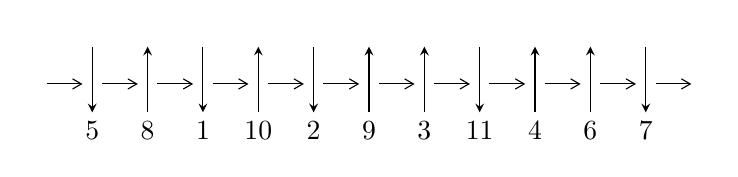
\begin{tikzpicture}[x=20pt, y=17pt]
	% nodes
	\node (C0) at (0, 0) {};
	\node (C1) at (1, 0) {};
	\node (C1U) at (1, +1) {};
	\node (C1D) at (1, -1) {5};

	\node (C2) at (2, 0) {};
	\node (C2U) at (2, +1) {};
	\node (C2D) at (2, -1) {8};

	\node (C3) at (3, 0) {};
	\node (C3U) at (3, +1) {};
	\node (C3D) at (3, -1) {1};

	\node (C4) at (4, 0) {};
	\node (C4U) at (4, +1) {};
	\node (C4D) at (4, -1) {10};

	\node (C5) at (5, 0) {};
	\node (C5U) at (5, +1) {};
	\node (C5D) at (5, -1) {2};

	\node (C6) at (6, 0) {};
	\node (C6U) at (6, +1) {};
	\node (C6D) at (6, -1) {9};

	\node (C7) at (7, 0) {};
	\node (C7U) at (7, +1) {};
	\node (C7D) at (7, -1) {3};

	\node (C8) at (8, 0) {};
	\node (C8U) at (8, +1) {};
	\node (C8D) at (8, -1) {11};

	\node (C9) at (9, 0) {};
	\node (C9U) at (9, +1) {};
	\node (C9D) at (9, -1) {4};

	\node (C10) at (10, 0) {};
	\node (C10U) at (10, +1) {};
	\node (C10D) at (10, -1) {6};

	\node (C11) at (11, 0) {};
	\node (C11U) at (11, +1) {};
	\node (C11D) at (11, -1) {7};
	\node (C12) at (12, 0) {};

	% arrows
	\draw[->,>={angle 60}]
	(C0) edge (C1) (C1) edge (C2) (C2) edge (C3) (C3) edge (C4) (C4) edge (C5) (C5) edge (C6) (C6) edge (C7) (C7) edge (C8) (C8) edge (C9) (C9) edge (C10) (C10) edge (C11) (C11) edge (C12) ;	\draw[->,>=stealth]
	(C1U) edge (C1D) (C2D) edge (C2U) (C3U) edge (C3D) (C4D) edge (C4U) (C5U) edge (C5D) (C6D) edge (C6U) (C7D) edge (C7U) (C8U) edge (C8D) (C9D) edge (C9U) (C10D) edge (C10U) (C11U) edge (C11D) ;
	\end{tikzpicture} \\
\hhline{~~} \\& 
\textbf{Solving Sequence} \\ \cline{2-2} 
 &
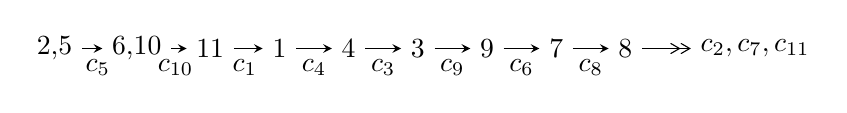
\begin{tikzpicture}[x=25pt, y=7pt]
	% node
	\node (A0) at (-1/8, 0) {2,5};
	\node (A1) at (17/16, 0) {6,10};
	\node (A2) at (17/8, 0) {11};
	\node (A3) at (25/8, 0) {1};
	\node (A4) at (33/8, 0) {4};
	\node (A5) at (41/8, 0) {3};
	\node (A6) at (49/8, 0) {9};
	\node (A7) at (57/8, 0) {7};
	\node (A8) at (65/8, 0) {8};
	\node (C1) at (1/2, -1) {$c_{5}$};
	\node (C2) at (13/8, -1) {$c_{10}$};
	\node (C3) at (21/8, -1) {$c_{1}$};
	\node (C4) at (29/8, -1) {$c_{4}$};
	\node (C5) at (37/8, -1) {$c_{3}$};
	\node (C6) at (45/8, -1) {$c_{9}$};
	\node (C7) at (53/8, -1) {$c_{6}$};
	\node (C8) at (61/8, -1) {$c_{8}$};
	\node (A9) at (10, 0) {$c_{2},c_{7},c_{11}$};

	% edge
	\draw[->,>=stealth]	
	(A0) edge (A1) (A1) edge (A2) (A2) edge (A3) (A3) edge (A4) (A4) edge (A5) (A5) edge (A6) (A6) edge (A7) (A7) edge (A8) ;
	\draw[->>,>={angle 60}]	
	(A8) edge (A9);
\end{tikzpicture} \\ 

\end{tabular} \\

\footnotetext{
The image of knot diagram is generated by the software ``\textbf{Draw programme}" developed by Andrew Bartholomew(\url{http://www.layer8.co.uk/maths/draw/index.htm\#Running-draw}), where we modified some parts for our purpose(\url{https://github.com/CATsTAILs/LinksPainter}).
}\phantom \\ \newline 
\centering \textbf{Ideals for irreducible components\footnotemark of $X_{\text{par}}$} 
 
\begin{align*}
I^u_{1}&=\langle 
3.70774\times10^{408} u^{106}+8.16968\times10^{408} u^{105}+\cdots+1.93043\times10^{406} b-5.29637\times10^{411},\\
\phantom{I^u_{1}}&\phantom{= \langle  }-1.82573\times10^{412} u^{106}-4.01506\times10^{412} u^{105}+\cdots+4.39752\times10^{409} a+2.56897\times10^{415},\\
\phantom{I^u_{1}}&\phantom{= \langle  }u^{107}+3 u^{106}+\cdots-10305 u-1139\rangle \\
I^u_{2}&=\langle 
244966793 u^{24}-694692620 u^{23}+\cdots+130021567 b-164391945,\\
\phantom{I^u_{2}}&\phantom{= \langle  }-9288763323 u^{24}+21892602582 u^{23}+\cdots+130021567 a+11899834301,\\
\phantom{I^u_{2}}&\phantom{= \langle  }u^{25}-2 u^{24}+\cdots+2 u-1\rangle \\
\\
\end{align*}
\raggedright * 2 irreducible components of $\dim_{\mathbb{C}}=0$, with total 132 representations.\\
\footnotetext{All coefficients of polynomials are rational numbers. But the coefficients are sometimes approximated in decimal forms when there is not enough margin.}
\newpage
\renewcommand{\arraystretch}{1}
\centering \section*{I. $I^u_{1}= \langle 3.71\times10^{408} u^{106}+8.17\times10^{408} u^{105}+\cdots+1.93\times10^{406} b-5.30\times10^{411},\;-1.83\times10^{412} u^{106}-4.02\times10^{412} u^{105}+\cdots+4.40\times10^{409} a+2.57\times10^{415},\;u^{107}+3 u^{106}+\cdots-10305 u-1139 \rangle$}
\flushleft \textbf{(i) Arc colorings}\\
\begin{tabular}{m{7pt} m{180pt} m{7pt} m{180pt} }
\flushright $a_{2}=$&$\begin{pmatrix}0\\u\end{pmatrix}$ \\
\flushright $a_{5}=$&$\begin{pmatrix}1\\0\end{pmatrix}$ \\
\flushright $a_{6}=$&$\begin{pmatrix}1\\u^2\end{pmatrix}$ \\
\flushright $a_{10}=$&$\begin{pmatrix}415.172 u^{106}+913.027 u^{105}+\cdots-4.57425\times10^{6} u-584186.\\-192.068 u^{106}-423.205 u^{105}+\cdots+2.13856\times10^{6} u+274362.\end{pmatrix}$ \\
\flushright $a_{11}=$&$\begin{pmatrix}-41.0477 u^{106}-94.0550 u^{105}+\cdots+517727. u+68881.1\\-477.753 u^{106}-1055.09 u^{105}+\cdots+5.34498\times10^{6} u+686198.\end{pmatrix}$ \\
\flushright $a_{1}=$&$\begin{pmatrix}u\\u\end{pmatrix}$ \\
\flushright $a_{4}=$&$\begin{pmatrix}-427.110 u^{106}-949.021 u^{105}+\cdots+4.83420\times10^{6} u+621333.\\453.142 u^{106}+1002.58 u^{105}+\cdots-5.09478\times10^{6} u-654884.\end{pmatrix}$ \\
\flushright $a_{3}=$&$\begin{pmatrix}110.931 u^{106}+246.015 u^{105}+\cdots-1.26496\times10^{6} u-163618.\\991.184 u^{106}+2197.61 u^{105}+\cdots-1.11939\times10^{7} u-1.43983\times10^{6}\end{pmatrix}$ \\
\flushright $a_{9}=$&$\begin{pmatrix}95.8929 u^{106}+194.195 u^{105}+\cdots-843416. u-101512.\\572.889 u^{106}+1274.47 u^{105}+\cdots-6.52524\times10^{6} u-840913.\end{pmatrix}$ \\
\flushright $a_{7}=$&$\begin{pmatrix}-90.0069 u^{106}-202.051 u^{105}+\cdots+1.05741\times10^{6} u+137578.\\-743.527 u^{106}-1660.72 u^{105}+\cdots+8.55566\times10^{6} u+1.10499\times10^{6}\end{pmatrix}$ \\
\flushright $a_{8}=$&$\begin{pmatrix}568.863 u^{106}+1271.75 u^{105}+\cdots-6.57032\times10^{6} u-849767.\\1649.37 u^{106}+3705.88 u^{105}+\cdots-1.92517\times10^{7} u-2.49360\times10^{6}\end{pmatrix}$\\ \flushright $a_{8}=$&$\begin{pmatrix}568.863 u^{106}+1271.75 u^{105}+\cdots-6.57032\times10^{6} u-849767.\\1649.37 u^{106}+3705.88 u^{105}+\cdots-1.92517\times10^{7} u-2.49360\times10^{6}\end{pmatrix}$\\&\end{tabular}
\flushleft \textbf{(ii) Obstruction class $= -1$}\\~\\
\flushleft \textbf{(iii) Cusp Shapes $= -912.136 u^{106}-2056.39 u^{105}+\cdots+1.07260\times10^{7} u+1.39093\times10^{6}$}\\~\\
\newpage\renewcommand{\arraystretch}{1}
\flushleft \textbf{(iv) u-Polynomials at the component}\newline \\
\begin{tabular}{m{50pt}|m{274pt}}
Crossings & \hspace{64pt}u-Polynomials at each crossing \\
\hline $$\begin{aligned}c_{1},c_{5}\end{aligned}$$&$\begin{aligned}
&u^{107}+3 u^{106}+\cdots-10305 u-1139
\end{aligned}$\\
\hline $$\begin{aligned}c_{2},c_{7}\end{aligned}$$&$\begin{aligned}
&u^{107}+u^{106}+\cdots-73 u+151
\end{aligned}$\\
\hline $$\begin{aligned}c_{3}\end{aligned}$$&$\begin{aligned}
&u^{107}-6 u^{106}+\cdots-6634767 u+1340716
\end{aligned}$\\
\hline $$\begin{aligned}c_{4},c_{9}\end{aligned}$$&$\begin{aligned}
&u^{107}+2 u^{106}+\cdots+282 u+193
\end{aligned}$\\
\hline $$\begin{aligned}c_{6}\end{aligned}$$&$\begin{aligned}
&u^{107}+16 u^{106}+\cdots-24 u-4
\end{aligned}$\\
\hline $$\begin{aligned}c_{8}\end{aligned}$$&$\begin{aligned}
&u^{107}-8 u^{106}+\cdots+29 u-2
\end{aligned}$\\
\hline $$\begin{aligned}c_{10}\end{aligned}$$&$\begin{aligned}
&u^{107}-2 u^{106}+\cdots-10504 u+844
\end{aligned}$\\
\hline $$\begin{aligned}c_{11}\end{aligned}$$&$\begin{aligned}
&u^{107}+2 u^{106}+\cdots-26229 u-6833
\end{aligned}$\\
\hline
\end{tabular}\\~\\
\newpage\renewcommand{\arraystretch}{1}
\flushleft \textbf{(v) Riley Polynomials at the component}\newline \\
\begin{tabular}{m{50pt}|m{274pt}}
Crossings & \hspace{64pt}Riley Polynomials at each crossing \\
\hline $$\begin{aligned}c_{1},c_{5}\end{aligned}$$&$\begin{aligned}
&y^{107}-55 y^{106}+\cdots+22754441 y-1297321
\end{aligned}$\\
\hline $$\begin{aligned}c_{2},c_{7}\end{aligned}$$&$\begin{aligned}
&y^{107}+75 y^{106}+\cdots-624341 y-22801
\end{aligned}$\\
\hline $$\begin{aligned}c_{3}\end{aligned}$$&$\begin{aligned}
&y^{107}-24 y^{106}+\cdots+2724074633153 y-1797519392656
\end{aligned}$\\
\hline $$\begin{aligned}c_{4},c_{9}\end{aligned}$$&$\begin{aligned}
&y^{107}-58 y^{106}+\cdots+979290 y-37249
\end{aligned}$\\
\hline $$\begin{aligned}c_{6}\end{aligned}$$&$\begin{aligned}
&y^{107}-6 y^{106}+\cdots+664 y-16
\end{aligned}$\\
\hline $$\begin{aligned}c_{8}\end{aligned}$$&$\begin{aligned}
&y^{107}-16 y^{106}+\cdots-35 y-4
\end{aligned}$\\
\hline $$\begin{aligned}c_{10}\end{aligned}$$&$\begin{aligned}
&y^{107}-4 y^{106}+\cdots+49093376 y-712336
\end{aligned}$\\
\hline $$\begin{aligned}c_{11}\end{aligned}$$&$\begin{aligned}
&y^{107}-16 y^{106}+\cdots+957467627 y-46689889
\end{aligned}$\\
\hline
\end{tabular}\\~\\
\newpage\flushleft \textbf{(vi) Complex Volumes and Cusp Shapes}
$$\begin{array}{c|c|c}  
\text{Solutions to }I^u_{1}& \I (\text{vol} + \sqrt{-1}CS) & \text{Cusp shape}\\
 \hline 
\begin{aligned}
u &= \phantom{-}0.986400 + 0.232370 I \\
a &= \phantom{-}0.94892 + 1.81516 I \\
b &= \phantom{-}0.26348 + 1.64192 I\end{aligned}
 & -7.68063 - 0.83209 I & \phantom{-0.000000 } 0 \\ \hline\begin{aligned}
u &= \phantom{-}0.986400 - 0.232370 I \\
a &= \phantom{-}0.94892 - 1.81516 I \\
b &= \phantom{-}0.26348 - 1.64192 I\end{aligned}
 & -7.68063 + 0.83209 I & \phantom{-0.000000 } 0 \\ \hline\begin{aligned}
u &= \phantom{-}0.942762 + 0.377969 I \\
a &= \phantom{-}0.75110 + 1.67803 I \\
b &= -0.961631 + 0.436996 I\end{aligned}
 & -1.71347 - 4.27371 I & \phantom{-0.000000 } 0 \\ \hline\begin{aligned}
u &= \phantom{-}0.942762 - 0.377969 I \\
a &= \phantom{-}0.75110 - 1.67803 I \\
b &= -0.961631 - 0.436996 I\end{aligned}
 & -1.71347 + 4.27371 I & \phantom{-0.000000 } 0 \\ \hline\begin{aligned}
u &= -0.958354 + 0.075778 I \\
a &= -0.10373 - 1.63196 I \\
b &= \phantom{-}1.149760 - 0.565303 I\end{aligned}
 & -3.40971 + 0.41855 I & \phantom{-0.000000 } 0 \\ \hline\begin{aligned}
u &= -0.958354 - 0.075778 I \\
a &= -0.10373 + 1.63196 I \\
b &= \phantom{-}1.149760 + 0.565303 I\end{aligned}
 & -3.40971 - 0.41855 I & \phantom{-0.000000 } 0 \\ \hline\begin{aligned}
u &= -0.779316 + 0.696451 I \\
a &= -0.504398 + 0.453268 I \\
b &= -0.971305 + 0.384066 I\end{aligned}
 & \phantom{-}0.10272 + 2.36255 I & \phantom{-0.000000 } 0 \\ \hline\begin{aligned}
u &= -0.779316 - 0.696451 I \\
a &= -0.504398 - 0.453268 I \\
b &= -0.971305 - 0.384066 I\end{aligned}
 & \phantom{-}0.10272 - 2.36255 I & \phantom{-0.000000 } 0 \\ \hline\begin{aligned}
u &= \phantom{-}0.177444 + 1.042760 I \\
a &= \phantom{-}0.1006440 - 0.0606927 I \\
b &= -1.185950 - 0.430093 I\end{aligned}
 & \phantom{-}3.78600 + 6.43458 I & \phantom{-0.000000 } 0 \\ \hline\begin{aligned}
u &= \phantom{-}0.177444 - 1.042760 I \\
a &= \phantom{-}0.1006440 + 0.0606927 I \\
b &= -1.185950 + 0.430093 I\end{aligned}
 & \phantom{-}3.78600 - 6.43458 I & \phantom{-0.000000 } 0\\
 \hline 
 \end{array}$$\newpage$$\begin{array}{c|c|c}  
\text{Solutions to }I^u_{1}& \I (\text{vol} + \sqrt{-1}CS) & \text{Cusp shape}\\
 \hline 
\begin{aligned}
u &= -0.895161 + 0.290884 I \\
a &= \phantom{-}0.505776 + 0.140299 I \\
b &= \phantom{-}1.68447 - 0.12670 I\end{aligned}
 & \phantom{-}0.58435 + 6.31456 I & \phantom{-0.000000 } 0 \\ \hline\begin{aligned}
u &= -0.895161 - 0.290884 I \\
a &= \phantom{-}0.505776 - 0.140299 I \\
b &= \phantom{-}1.68447 + 0.12670 I\end{aligned}
 & \phantom{-}0.58435 - 6.31456 I & \phantom{-0.000000 } 0 \\ \hline\begin{aligned}
u &= -1.015630 + 0.422544 I \\
a &= -0.608996 + 1.091860 I \\
b &= -0.298045 + 0.748953 I\end{aligned}
 & -1.73579 + 1.74529 I & \phantom{-0.000000 } 0 \\ \hline\begin{aligned}
u &= -1.015630 - 0.422544 I \\
a &= -0.608996 - 1.091860 I \\
b &= -0.298045 - 0.748953 I\end{aligned}
 & -1.73579 - 1.74529 I & \phantom{-0.000000 } 0 \\ \hline\begin{aligned}
u &= \phantom{-}0.504244 + 0.740958 I \\
a &= -0.0333710 + 0.0042260 I \\
b &= \phantom{-}1.121870 + 0.369553 I\end{aligned}
 & \phantom{-}2.26806 + 1.29518 I & \phantom{-0.000000 } 0 \\ \hline\begin{aligned}
u &= \phantom{-}0.504244 - 0.740958 I \\
a &= -0.0333710 - 0.0042260 I \\
b &= \phantom{-}1.121870 - 0.369553 I\end{aligned}
 & \phantom{-}2.26806 - 1.29518 I & \phantom{-0.000000 } 0 \\ \hline\begin{aligned}
u &= \phantom{-}1.026430 + 0.445067 I \\
a &= \phantom{-}0.50031 - 1.38036 I \\
b &= \phantom{-}1.221760 - 0.462110 I\end{aligned}
 & \phantom{-}3.45857 - 2.35544 I & \phantom{-0.000000 } 0 \\ \hline\begin{aligned}
u &= \phantom{-}1.026430 - 0.445067 I \\
a &= \phantom{-}0.50031 + 1.38036 I \\
b &= \phantom{-}1.221760 + 0.462110 I\end{aligned}
 & \phantom{-}3.45857 + 2.35544 I & \phantom{-0.000000 } 0 \\ \hline\begin{aligned}
u &= -0.013670 + 0.872769 I \\
a &= -1.057650 - 0.304944 I \\
b &= \phantom{-}0.199244 - 0.708064 I\end{aligned}
 & -2.93156 + 7.07012 I & \phantom{-0.000000 } 0 \\ \hline\begin{aligned}
u &= -0.013670 - 0.872769 I \\
a &= -1.057650 + 0.304944 I \\
b &= \phantom{-}0.199244 + 0.708064 I\end{aligned}
 & -2.93156 - 7.07012 I & \phantom{-0.000000 } 0\\
 \hline 
 \end{array}$$\newpage$$\begin{array}{c|c|c}  
\text{Solutions to }I^u_{1}& \I (\text{vol} + \sqrt{-1}CS) & \text{Cusp shape}\\
 \hline 
\begin{aligned}
u &= \phantom{-}1.038590 + 0.476453 I \\
a &= -0.22479 + 2.27046 I \\
b &= -1.228310 + 0.377670 I\end{aligned}
 & \phantom{-}0.79397 - 8.09835 I & \phantom{-0.000000 } 0 \\ \hline\begin{aligned}
u &= \phantom{-}1.038590 - 0.476453 I \\
a &= -0.22479 - 2.27046 I \\
b &= -1.228310 - 0.377670 I\end{aligned}
 & \phantom{-}0.79397 + 8.09835 I & \phantom{-0.000000 } 0 \\ \hline\begin{aligned}
u &= \phantom{-}0.992427 + 0.582979 I \\
a &= \phantom{-}0.28613 + 1.52727 I \\
b &= -0.804721 + 0.144032 I\end{aligned}
 & -0.60216 - 4.42014 I & \phantom{-0.000000 } 0 \\ \hline\begin{aligned}
u &= \phantom{-}0.992427 - 0.582979 I \\
a &= \phantom{-}0.28613 - 1.52727 I \\
b &= -0.804721 - 0.144032 I\end{aligned}
 & -0.60216 + 4.42014 I & \phantom{-0.000000 } 0 \\ \hline\begin{aligned}
u &= -0.528391 + 0.662505 I \\
a &= -0.525822 + 0.658236 I \\
b &= -0.258034 + 0.406970 I\end{aligned}
 & -0.57780 + 2.21426 I & \phantom{-0.000000 } 0 \\ \hline\begin{aligned}
u &= -0.528391 - 0.662505 I \\
a &= -0.525822 - 0.658236 I \\
b &= -0.258034 - 0.406970 I\end{aligned}
 & -0.57780 - 2.21426 I & \phantom{-0.000000 } 0 \\ \hline\begin{aligned}
u &= -0.758270 + 0.377359 I \\
a &= -0.97768 - 1.94616 I \\
b &= -1.200130 - 0.362063 I\end{aligned}
 & \phantom{-}0.87955 - 3.38375 I & \phantom{-0.000000 } 0 \\ \hline\begin{aligned}
u &= -0.758270 - 0.377359 I \\
a &= -0.97768 + 1.94616 I \\
b &= -1.200130 + 0.362063 I\end{aligned}
 & \phantom{-}0.87955 + 3.38375 I & \phantom{-0.000000 } 0 \\ \hline\begin{aligned}
u &= \phantom{-}0.317941 + 0.777701 I \\
a &= \phantom{-}0.113685 + 0.456499 I \\
b &= -1.271250 - 0.022410 I\end{aligned}
 & \phantom{-}5.70627 - 2.04309 I & \phantom{-0.000000 } 0 \\ \hline\begin{aligned}
u &= \phantom{-}0.317941 - 0.777701 I \\
a &= \phantom{-}0.113685 - 0.456499 I \\
b &= -1.271250 + 0.022410 I\end{aligned}
 & \phantom{-}5.70627 + 2.04309 I & \phantom{-0.000000 } 0\\
 \hline 
 \end{array}$$\newpage$$\begin{array}{c|c|c}  
\text{Solutions to }I^u_{1}& \I (\text{vol} + \sqrt{-1}CS) & \text{Cusp shape}\\
 \hline 
\begin{aligned}
u &= -1.141690 + 0.244876 I \\
a &= \phantom{-}1.11712 + 1.68774 I \\
b &= \phantom{-}1.074340 + 0.337271 I\end{aligned}
 & \phantom{-}1.05453 + 4.32890 I & \phantom{-0.000000 } 0 \\ \hline\begin{aligned}
u &= -1.141690 - 0.244876 I \\
a &= \phantom{-}1.11712 - 1.68774 I \\
b &= \phantom{-}1.074340 - 0.337271 I\end{aligned}
 & \phantom{-}1.05453 - 4.32890 I & \phantom{-0.000000 } 0 \\ \hline\begin{aligned}
u &= \phantom{-}1.172160 + 0.081485 I \\
a &= -0.09877 - 1.50658 I \\
b &= -0.366081 - 1.317570 I\end{aligned}
 & -8.46915 + 0.58647 I & \phantom{-0.000000 } 0 \\ \hline\begin{aligned}
u &= \phantom{-}1.172160 - 0.081485 I \\
a &= -0.09877 + 1.50658 I \\
b &= -0.366081 + 1.317570 I\end{aligned}
 & -8.46915 - 0.58647 I & \phantom{-0.000000 } 0 \\ \hline\begin{aligned}
u &= -1.125510 + 0.369873 I \\
a &= \phantom{-}0.49032 - 1.38272 I \\
b &= \phantom{-}0.390445 - 1.233280 I\end{aligned}
 & -2.50091 + 5.55154 I & \phantom{-0.000000 } 0 \\ \hline\begin{aligned}
u &= -1.125510 - 0.369873 I \\
a &= \phantom{-}0.49032 + 1.38272 I \\
b &= \phantom{-}0.390445 + 1.233280 I\end{aligned}
 & -2.50091 - 5.55154 I & \phantom{-0.000000 } 0 \\ \hline\begin{aligned}
u &= \phantom{-}0.967874 + 0.696932 I \\
a &= \phantom{-}0.13939 + 1.74328 I \\
b &= -1.066700 + 0.627717 I\end{aligned}
 & \phantom{-}0.84643 - 6.63458 I & \phantom{-0.000000 } 0 \\ \hline\begin{aligned}
u &= \phantom{-}0.967874 - 0.696932 I \\
a &= \phantom{-}0.13939 - 1.74328 I \\
b &= -1.066700 - 0.627717 I\end{aligned}
 & \phantom{-}0.84643 + 6.63458 I & \phantom{-0.000000 } 0 \\ \hline\begin{aligned}
u &= \phantom{-}0.583611 + 0.547652 I \\
a &= -0.811130 + 0.011218 I \\
b &= \phantom{-}1.388120 + 0.262275 I\end{aligned}
 & \phantom{-}2.21393 + 3.95320 I & \phantom{-0.000000 } 0 \\ \hline\begin{aligned}
u &= \phantom{-}0.583611 - 0.547652 I \\
a &= -0.811130 - 0.011218 I \\
b &= \phantom{-}1.388120 - 0.262275 I\end{aligned}
 & \phantom{-}2.21393 - 3.95320 I & \phantom{-0.000000 } 0\\
 \hline 
 \end{array}$$\newpage$$\begin{array}{c|c|c}  
\text{Solutions to }I^u_{1}& \I (\text{vol} + \sqrt{-1}CS) & \text{Cusp shape}\\
 \hline 
\begin{aligned}
u &= -0.795751 + 0.026610 I \\
a &= -1.46071 + 0.31634 I \\
b &= -0.570264 + 0.577089 I\end{aligned}
 & -3.11864 - 0.19481 I & \phantom{-0.000000 } 0 \\ \hline\begin{aligned}
u &= -0.795751 - 0.026610 I \\
a &= -1.46071 - 0.31634 I \\
b &= -0.570264 - 0.577089 I\end{aligned}
 & -3.11864 + 0.19481 I & \phantom{-0.000000 } 0 \\ \hline\begin{aligned}
u &= \phantom{-}0.777664 + 0.122407 I \\
a &= -0.65432 - 2.51164 I \\
b &= \phantom{-}0.648800 - 0.175263 I\end{aligned}
 & -0.59738 + 1.82584 I & \phantom{-0.000000 } 0 \\ \hline\begin{aligned}
u &= \phantom{-}0.777664 - 0.122407 I \\
a &= -0.65432 + 2.51164 I \\
b &= \phantom{-}0.648800 + 0.175263 I\end{aligned}
 & -0.59738 - 1.82584 I & \phantom{-0.000000 } 0 \\ \hline\begin{aligned}
u &= -1.215000 + 0.037952 I \\
a &= -0.818057 + 0.597206 I \\
b &= -0.458096 + 0.474076 I\end{aligned}
 & -3.11142 + 0.38976 I & \phantom{-0.000000 } 0 \\ \hline\begin{aligned}
u &= -1.215000 - 0.037952 I \\
a &= -0.818057 - 0.597206 I \\
b &= -0.458096 - 0.474076 I\end{aligned}
 & -3.11142 - 0.38976 I & \phantom{-0.000000 } 0 \\ \hline\begin{aligned}
u &= -1.001390 + 0.697728 I \\
a &= -0.743289 + 1.106810 I \\
b &= \phantom{-}0.700521 + 0.787341 I\end{aligned}
 & -4.48306 + 5.28560 I & \phantom{-0.000000 } 0 \\ \hline\begin{aligned}
u &= -1.001390 - 0.697728 I \\
a &= -0.743289 - 1.106810 I \\
b &= \phantom{-}0.700521 - 0.787341 I\end{aligned}
 & -4.48306 - 5.28560 I & \phantom{-0.000000 } 0 \\ \hline\begin{aligned}
u &= -0.541425 + 0.553774 I \\
a &= -0.384506 - 0.148529 I \\
b &= -0.356617 + 0.793713 I\end{aligned}
 & -3.48677 - 0.29528 I & \phantom{-0.000000 } 0 \\ \hline\begin{aligned}
u &= -0.541425 - 0.553774 I \\
a &= -0.384506 + 0.148529 I \\
b &= -0.356617 - 0.793713 I\end{aligned}
 & -3.48677 + 0.29528 I & \phantom{-0.000000 } 0\\
 \hline 
 \end{array}$$\newpage$$\begin{array}{c|c|c}  
\text{Solutions to }I^u_{1}& \I (\text{vol} + \sqrt{-1}CS) & \text{Cusp shape}\\
 \hline 
\begin{aligned}
u &= -0.760332 + 0.012943 I \\
a &= \phantom{-}0.855839 - 0.321413 I \\
b &= -1.396060 + 0.132482 I\end{aligned}
 & \phantom{-}3.02312 - 3.08803 I & \phantom{-0.000000 } 0 \\ \hline\begin{aligned}
u &= -0.760332 - 0.012943 I \\
a &= \phantom{-}0.855839 + 0.321413 I \\
b &= -1.396060 - 0.132482 I\end{aligned}
 & \phantom{-}3.02312 + 3.08803 I & \phantom{-0.000000 } 0 \\ \hline\begin{aligned}
u &= \phantom{-}0.670518 + 0.345863 I \\
a &= \phantom{-}1.23360 + 1.94436 I \\
b &= -0.972382 + 0.540863 I\end{aligned}
 & -1.90792 - 4.34721 I & \phantom{-0.000000 } 0 \\ \hline\begin{aligned}
u &= \phantom{-}0.670518 - 0.345863 I \\
a &= \phantom{-}1.23360 - 1.94436 I \\
b &= -0.972382 - 0.540863 I\end{aligned}
 & -1.90792 + 4.34721 I & \phantom{-0.000000 } 0 \\ \hline\begin{aligned}
u &= -1.138980 + 0.512959 I \\
a &= -0.05806 + 1.65313 I \\
b &= \phantom{-}1.41965 + 0.74374 I\end{aligned}
 & -3.66538 + 8.73172 I & \phantom{-0.000000 } 0 \\ \hline\begin{aligned}
u &= -1.138980 - 0.512959 I \\
a &= -0.05806 - 1.65313 I \\
b &= \phantom{-}1.41965 - 0.74374 I\end{aligned}
 & -3.66538 - 8.73172 I & \phantom{-0.000000 } 0 \\ \hline\begin{aligned}
u &= \phantom{-}0.491471 + 1.150150 I \\
a &= -0.312123 + 0.353998 I \\
b &= \phantom{-}1.075750 + 0.300107 I\end{aligned}
 & \phantom{-}2.80517 + 0.25289 I & \phantom{-0.000000 } 0 \\ \hline\begin{aligned}
u &= \phantom{-}0.491471 - 1.150150 I \\
a &= -0.312123 - 0.353998 I \\
b &= \phantom{-}1.075750 - 0.300107 I\end{aligned}
 & \phantom{-}2.80517 - 0.25289 I & \phantom{-0.000000 } 0 \\ \hline\begin{aligned}
u &= \phantom{-}1.180050 + 0.415213 I \\
a &= \phantom{-}0.506233 + 0.429519 I \\
b &= \phantom{-}0.749302 + 0.843791 I\end{aligned}
 & -4.38972 + 0.65205 I & \phantom{-0.000000 } 0 \\ \hline\begin{aligned}
u &= \phantom{-}1.180050 - 0.415213 I \\
a &= \phantom{-}0.506233 - 0.429519 I \\
b &= \phantom{-}0.749302 - 0.843791 I\end{aligned}
 & -4.38972 - 0.65205 I & \phantom{-0.000000 } 0\\
 \hline 
 \end{array}$$\newpage$$\begin{array}{c|c|c}  
\text{Solutions to }I^u_{1}& \I (\text{vol} + \sqrt{-1}CS) & \text{Cusp shape}\\
 \hline 
\begin{aligned}
u &= -1.216470 + 0.294723 I \\
a &= -0.71129 + 1.56282 I \\
b &= \phantom{-}1.095460 + 0.361300 I\end{aligned}
 & -5.13584 + 7.74504 I & \phantom{-0.000000 } 0 \\ \hline\begin{aligned}
u &= -1.216470 - 0.294723 I \\
a &= -0.71129 - 1.56282 I \\
b &= \phantom{-}1.095460 - 0.361300 I\end{aligned}
 & -5.13584 - 7.74504 I & \phantom{-0.000000 } 0 \\ \hline\begin{aligned}
u &= -0.597176 + 0.450609 I \\
a &= -0.18481 + 1.97419 I \\
b &= \phantom{-}0.719013 + 0.729095 I\end{aligned}
 & \phantom{-}0.69488 + 2.31741 I & \phantom{-0.000000 } 0 \\ \hline\begin{aligned}
u &= -0.597176 - 0.450609 I \\
a &= -0.18481 - 1.97419 I \\
b &= \phantom{-}0.719013 - 0.729095 I\end{aligned}
 & \phantom{-}0.69488 - 2.31741 I & \phantom{-0.000000 } 0 \\ \hline\begin{aligned}
u &= \phantom{-}0.747034\phantom{ +0.000000I} \\
a &= -0.985560\phantom{ +0.000000I} \\
b &= -1.81420\phantom{ +0.000000I}\end{aligned}
 & \phantom{-}6.04974\phantom{ +0.000000I} & \phantom{-0.000000 } 0 \\ \hline\begin{aligned}
u &= \phantom{-}0.783338 + 1.031040 I \\
a &= -0.476712 - 0.175098 I \\
b &= \phantom{-}1.054390 - 0.258775 I\end{aligned}
 & \phantom{-}0.222061 - 0.979752 I & \phantom{-0.000000 } 0 \\ \hline\begin{aligned}
u &= \phantom{-}0.783338 - 1.031040 I \\
a &= -0.476712 + 0.175098 I \\
b &= \phantom{-}1.054390 + 0.258775 I\end{aligned}
 & \phantom{-}0.222061 + 0.979752 I & \phantom{-0.000000 } 0 \\ \hline\begin{aligned}
u &= \phantom{-}1.129370 + 0.667915 I \\
a &= \phantom{-}0.04446 + 1.66659 I \\
b &= -1.138630 + 0.569880 I\end{aligned}
 & \phantom{-}0.71143 - 6.72557 I & \phantom{-0.000000 } 0 \\ \hline\begin{aligned}
u &= \phantom{-}1.129370 - 0.667915 I \\
a &= \phantom{-}0.04446 - 1.66659 I \\
b &= -1.138630 - 0.569880 I\end{aligned}
 & \phantom{-}0.71143 + 6.72557 I & \phantom{-0.000000 } 0 \\ \hline\begin{aligned}
u &= -0.306453 + 1.281190 I \\
a &= -0.179496 - 0.169731 I \\
b &= \phantom{-}1.160100 - 0.518560 I\end{aligned}
 & -0.15826 - 11.75880 I & \phantom{-0.000000 } 0\\
 \hline 
 \end{array}$$\newpage$$\begin{array}{c|c|c}  
\text{Solutions to }I^u_{1}& \I (\text{vol} + \sqrt{-1}CS) & \text{Cusp shape}\\
 \hline 
\begin{aligned}
u &= -0.306453 - 1.281190 I \\
a &= -0.179496 + 0.169731 I \\
b &= \phantom{-}1.160100 + 0.518560 I\end{aligned}
 & -0.15826 + 11.75880 I & \phantom{-0.000000 } 0 \\ \hline\begin{aligned}
u &= -0.256265 + 0.616203 I \\
a &= \phantom{-}0.659506 - 0.891867 I \\
b &= -1.174010 + 0.469012 I\end{aligned}
 & -1.10598 - 4.23301 I & \phantom{-0.000000 } 0 \\ \hline\begin{aligned}
u &= -0.256265 - 0.616203 I \\
a &= \phantom{-}0.659506 + 0.891867 I \\
b &= -1.174010 - 0.469012 I\end{aligned}
 & -1.10598 + 4.23301 I & \phantom{-0.000000 } 0 \\ \hline\begin{aligned}
u &= \phantom{-}1.249560 + 0.496859 I \\
a &= -0.470769 - 1.167780 I \\
b &= -0.303354 - 1.221520 I\end{aligned}
 & -6.63108 - 11.96940 I & \phantom{-0.000000 } 0 \\ \hline\begin{aligned}
u &= \phantom{-}1.249560 - 0.496859 I \\
a &= -0.470769 + 1.167780 I \\
b &= -0.303354 + 1.221520 I\end{aligned}
 & -6.63108 + 11.96940 I & \phantom{-0.000000 } 0 \\ \hline\begin{aligned}
u &= \phantom{-}1.309780 + 0.330332 I \\
a &= \phantom{-}0.274873 - 0.790752 I \\
b &= \phantom{-}0.089576 - 0.732286 I\end{aligned}
 & -6.27513 - 5.21106 I & \phantom{-0.000000 } 0 \\ \hline\begin{aligned}
u &= \phantom{-}1.309780 - 0.330332 I \\
a &= \phantom{-}0.274873 + 0.790752 I \\
b &= \phantom{-}0.089576 + 0.732286 I\end{aligned}
 & -6.27513 + 5.21106 I & \phantom{-0.000000 } 0 \\ \hline\begin{aligned}
u &= \phantom{-}1.339110 + 0.384317 I \\
a &= \phantom{-}0.218932 + 1.021670 I \\
b &= \phantom{-}0.428507 + 0.715696 I\end{aligned}
 & -3.42958 - 4.03082 I & \phantom{-0.000000 } 0 \\ \hline\begin{aligned}
u &= \phantom{-}1.339110 - 0.384317 I \\
a &= \phantom{-}0.218932 - 1.021670 I \\
b &= \phantom{-}0.428507 - 0.715696 I\end{aligned}
 & -3.42958 + 4.03082 I & \phantom{-0.000000 } 0 \\ \hline\begin{aligned}
u &= -0.596030 + 0.015402 I \\
a &= -1.40783 + 4.40453 I \\
b &= -0.624969 - 0.029942 I\end{aligned}
 & -2.33761 + 6.09907 I & \phantom{-0.000000 } 0\\
 \hline 
 \end{array}$$\newpage$$\begin{array}{c|c|c}  
\text{Solutions to }I^u_{1}& \I (\text{vol} + \sqrt{-1}CS) & \text{Cusp shape}\\
 \hline 
\begin{aligned}
u &= -0.596030 - 0.015402 I \\
a &= -1.40783 - 4.40453 I \\
b &= -0.624969 + 0.029942 I\end{aligned}
 & -2.33761 - 6.09907 I & \phantom{-0.000000 } 0 \\ \hline\begin{aligned}
u &= \phantom{-}1.278180 + 0.597403 I \\
a &= \phantom{-}0.16469 - 1.50384 I \\
b &= \phantom{-}1.27288 - 0.69832 I\end{aligned}
 & \phantom{-}0.38916 - 12.29960 I & \phantom{-0.000000 } 0 \\ \hline\begin{aligned}
u &= \phantom{-}1.278180 - 0.597403 I \\
a &= \phantom{-}0.16469 + 1.50384 I \\
b &= \phantom{-}1.27288 + 0.69832 I\end{aligned}
 & \phantom{-}0.38916 + 12.29960 I & \phantom{-0.000000 } 0 \\ \hline\begin{aligned}
u &= -1.34893 + 0.42751 I \\
a &= -0.341692 - 1.233990 I \\
b &= -1.26189 - 0.70892 I\end{aligned}
 & -5.54355 + 6.30492 I & \phantom{-0.000000 } 0 \\ \hline\begin{aligned}
u &= -1.34893 - 0.42751 I \\
a &= -0.341692 + 1.233990 I \\
b &= -1.26189 + 0.70892 I\end{aligned}
 & -5.54355 - 6.30492 I & \phantom{-0.000000 } 0 \\ \hline\begin{aligned}
u &= -1.36142 + 0.44294 I \\
a &= \phantom{-}0.344902 - 0.967409 I \\
b &= -0.886579 - 0.536312 I\end{aligned}
 & -6.97914 - 1.89469 I & \phantom{-0.000000 } 0 \\ \hline\begin{aligned}
u &= -1.36142 - 0.44294 I \\
a &= \phantom{-}0.344902 + 0.967409 I \\
b &= -0.886579 + 0.536312 I\end{aligned}
 & -6.97914 + 1.89469 I & \phantom{-0.000000 } 0 \\ \hline\begin{aligned}
u &= \phantom{-}1.46671 + 0.18400 I \\
a &= \phantom{-}0.997962 + 0.379768 I \\
b &= \phantom{-}0.537001 + 0.211295 I\end{aligned}
 & -7.13217 - 4.86452 I & \phantom{-0.000000 } 0 \\ \hline\begin{aligned}
u &= \phantom{-}1.46671 - 0.18400 I \\
a &= \phantom{-}0.997962 - 0.379768 I \\
b &= \phantom{-}0.537001 - 0.211295 I\end{aligned}
 & -7.13217 + 4.86452 I & \phantom{-0.000000 } 0 \\ \hline\begin{aligned}
u &= -0.25299 + 1.45770 I \\
a &= \phantom{-}0.371342 + 0.340879 I \\
b &= -0.889840 + 0.339869 I\end{aligned}
 & \phantom{-}2.73935 - 1.44205 I & \phantom{-0.000000 } 0\\
 \hline 
 \end{array}$$\newpage$$\begin{array}{c|c|c}  
\text{Solutions to }I^u_{1}& \I (\text{vol} + \sqrt{-1}CS) & \text{Cusp shape}\\
 \hline 
\begin{aligned}
u &= -0.25299 - 1.45770 I \\
a &= \phantom{-}0.371342 - 0.340879 I \\
b &= -0.889840 - 0.339869 I\end{aligned}
 & \phantom{-}2.73935 + 1.44205 I & \phantom{-0.000000 } 0 \\ \hline\begin{aligned}
u &= -1.32821 + 0.69461 I \\
a &= \phantom{-}0.01175 - 1.46223 I \\
b &= -1.29936 - 0.68644 I\end{aligned}
 & -3.4594 + 18.6505 I & \phantom{-0.000000 } 0 \\ \hline\begin{aligned}
u &= -1.32821 - 0.69461 I \\
a &= \phantom{-}0.01175 + 1.46223 I \\
b &= -1.29936 + 0.68644 I\end{aligned}
 & -3.4594 - 18.6505 I & \phantom{-0.000000 } 0 \\ \hline\begin{aligned}
u &= -1.30416 + 0.74302 I \\
a &= \phantom{-}0.222241 + 0.523886 I \\
b &= \phantom{-}0.781123 - 0.138371 I\end{aligned}
 & -0.983804 - 0.893136 I & \phantom{-0.000000 } 0 \\ \hline\begin{aligned}
u &= -1.30416 - 0.74302 I \\
a &= \phantom{-}0.222241 - 0.523886 I \\
b &= \phantom{-}0.781123 + 0.138371 I\end{aligned}
 & -0.983804 + 0.893136 I & \phantom{-0.000000 } 0 \\ \hline\begin{aligned}
u &= \phantom{-}0.065712 + 0.481544 I \\
a &= -0.052612 + 0.945417 I \\
b &= \phantom{-}0.334016 + 0.340844 I\end{aligned}
 & \phantom{-}0.707089 + 1.076880 I & \phantom{-}4.73200 - 5.26476 I \\ \hline\begin{aligned}
u &= \phantom{-}0.065712 - 0.481544 I \\
a &= -0.052612 - 0.945417 I \\
b &= \phantom{-}0.334016 - 0.340844 I\end{aligned}
 & \phantom{-}0.707089 - 1.076880 I & \phantom{-}4.73200 + 5.26476 I \\ \hline\begin{aligned}
u &= -1.31792 + 0.78965 I \\
a &= \phantom{-}0.106183 - 0.905562 I \\
b &= -1.221770 - 0.464344 I\end{aligned}
 & -2.61168 + 9.55584 I & \phantom{-0.000000 } 0 \\ \hline\begin{aligned}
u &= -1.31792 - 0.78965 I \\
a &= \phantom{-}0.106183 + 0.905562 I \\
b &= -1.221770 + 0.464344 I\end{aligned}
 & -2.61168 - 9.55584 I & \phantom{-0.000000 } 0 \\ \hline\begin{aligned}
u &= -1.45253 + 0.66887 I \\
a &= \phantom{-}0.044860 + 1.310230 I \\
b &= \phantom{-}1.088320 + 0.554757 I\end{aligned}
 & -1.44975 + 8.88875 I & \phantom{-0.000000 } 0\\
 \hline 
 \end{array}$$\newpage$$\begin{array}{c|c|c}  
\text{Solutions to }I^u_{1}& \I (\text{vol} + \sqrt{-1}CS) & \text{Cusp shape}\\
 \hline 
\begin{aligned}
u &= -1.45253 - 0.66887 I \\
a &= \phantom{-}0.044860 - 1.310230 I \\
b &= \phantom{-}1.088320 - 0.554757 I\end{aligned}
 & -1.44975 - 8.88875 I & \phantom{-0.000000 } 0 \\ \hline\begin{aligned}
u &= -0.146393 + 0.303286 I \\
a &= \phantom{-}2.33022 - 1.64478 I \\
b &= \phantom{-}0.121707 - 0.702495 I\end{aligned}
 & \phantom{-}0.20217 - 2.39762 I & \phantom{-}2.80067 + 2.93719 I \\ \hline\begin{aligned}
u &= -0.146393 - 0.303286 I \\
a &= \phantom{-}2.33022 + 1.64478 I \\
b &= \phantom{-}0.121707 + 0.702495 I\end{aligned}
 & \phantom{-}0.20217 + 2.39762 I & \phantom{-}2.80067 - 2.93719 I \\ \hline\begin{aligned}
u &= \phantom{-}1.67278 + 0.07424 I \\
a &= -0.302795 - 0.461913 I \\
b &= -0.675695 - 0.428254 I\end{aligned}
 & -7.67236 + 5.96387 I & \phantom{-0.000000 } 0 \\ \hline\begin{aligned}
u &= \phantom{-}1.67278 - 0.07424 I \\
a &= -0.302795 + 0.461913 I \\
b &= -0.675695 + 0.428254 I\end{aligned}
 & -7.67236 - 5.96387 I & \phantom{-0.000000 } 0 \\ \hline\begin{aligned}
u &= \phantom{-}0.15618 + 1.97729 I \\
a &= -0.202346 + 0.018617 I \\
b &= \phantom{-}0.979165 - 0.204325 I\end{aligned}
 & \phantom{-}0.116311 - 0.699806 I & \phantom{-0.000000 } 0 \\ \hline\begin{aligned}
u &= \phantom{-}0.15618 - 1.97729 I \\
a &= -0.202346 - 0.018617 I \\
b &= \phantom{-}0.979165 + 0.204325 I\end{aligned}
 & \phantom{-}0.116311 + 0.699806 I & \phantom{-0.000000 } 0\\
 \hline 
 \end{array}$$\newpage\newpage\renewcommand{\arraystretch}{1}
\centering \section*{II. $I^u_{2}= \langle 2.45\times10^{8} u^{24}-6.95\times10^{8} u^{23}+\cdots+1.30\times10^{8} b-1.64\times10^{8},\;-9.29\times10^{9} u^{24}+2.19\times10^{10} u^{23}+\cdots+1.30\times10^{8} a+1.19\times10^{10},\;u^{25}-2 u^{24}+\cdots+2 u-1 \rangle$}
\flushleft \textbf{(i) Arc colorings}\\
\begin{tabular}{m{7pt} m{180pt} m{7pt} m{180pt} }
\flushright $a_{2}=$&$\begin{pmatrix}0\\u\end{pmatrix}$ \\
\flushright $a_{5}=$&$\begin{pmatrix}1\\0\end{pmatrix}$ \\
\flushright $a_{6}=$&$\begin{pmatrix}1\\u^2\end{pmatrix}$ \\
\flushright $a_{10}=$&$\begin{pmatrix}71.4402 u^{24}-168.377 u^{23}+\cdots+422.826 u-91.5220\\-1.88405 u^{24}+5.34290 u^{23}+\cdots-3.00018 u+1.26434\end{pmatrix}$ \\
\flushright $a_{11}=$&$\begin{pmatrix}50.4042 u^{24}-117.902 u^{23}+\cdots+297.393 u-64.7613\\-6.41737 u^{24}+16.7357 u^{23}+\cdots-40.8416 u+9.66707\end{pmatrix}$ \\
\flushright $a_{1}=$&$\begin{pmatrix}u\\u\end{pmatrix}$ \\
\flushright $a_{4}=$&$\begin{pmatrix}-68.2812 u^{24}+196.749 u^{23}+\cdots-644.811 u+193.281\\5.42990 u^{24}-8.79498 u^{23}+\cdots+6.33272 u+1.18076\end{pmatrix}$ \\
\flushright $a_{3}=$&$\begin{pmatrix}-46.8507 u^{24}+136.870 u^{23}+\cdots-454.856 u+135.159\\26.8603 u^{24}-68.6734 u^{23}+\cdots+196.287 u-56.9409\end{pmatrix}$ \\
\flushright $a_{9}=$&$\begin{pmatrix}-87.1836 u^{24}+196.568 u^{23}+\cdots-462.463 u+90.7930\\-6.36834 u^{24}+4.10518 u^{23}+\cdots+20.5737 u-14.0614\end{pmatrix}$ \\
\flushright $a_{7}=$&$\begin{pmatrix}-29.2290 u^{24}+42.9489 u^{23}+\cdots+14.6771 u-43.1831\\-53.9897 u^{24}+114.506 u^{23}+\cdots-233.641 u+43.7286\end{pmatrix}$ \\
\flushright $a_{8}=$&$\begin{pmatrix}67.2328 u^{24}-185.134 u^{23}+\cdots+569.048 u-172.843\\58.0366 u^{24}-151.454 u^{23}+\cdots+442.251 u-101.964\end{pmatrix}$\\ \flushright $a_{8}=$&$\begin{pmatrix}67.2328 u^{24}-185.134 u^{23}+\cdots+569.048 u-172.843\\58.0366 u^{24}-151.454 u^{23}+\cdots+442.251 u-101.964\end{pmatrix}$\\&\end{tabular}
\flushleft \textbf{(ii) Obstruction class $= 1$}\\~\\
\flushleft \textbf{(iii) Cusp Shapes $= -\frac{19591815370}{130021567} u^{24}+\frac{57307936648}{130021567} u^{23}+\cdots-\frac{190001294619}{130021567} u+\frac{61319203002}{130021567}$}\\~\\
\newpage\renewcommand{\arraystretch}{1}
\flushleft \textbf{(iv) u-Polynomials at the component}\newline \\
\begin{tabular}{m{50pt}|m{274pt}}
Crossings & \hspace{64pt}u-Polynomials at each crossing \\
\hline $$\begin{aligned}c_{1}\end{aligned}$$&$\begin{aligned}
&u^{25}+2 u^{24}+\cdots+2 u+1
\end{aligned}$\\
\hline $$\begin{aligned}c_{2}\end{aligned}$$&$\begin{aligned}
&u^{25}+11 u^{23}+\cdots-8 u^2-1
\end{aligned}$\\
\hline $$\begin{aligned}c_{3}\end{aligned}$$&$\begin{aligned}
&u^{25}+5 u^{24}+\cdots+58 u+1
\end{aligned}$\\
\hline $$\begin{aligned}c_{4}\end{aligned}$$&$\begin{aligned}
&u^{25}- u^{24}+\cdots+u-1
\end{aligned}$\\
\hline $$\begin{aligned}c_{5}\end{aligned}$$&$\begin{aligned}
&u^{25}-2 u^{24}+\cdots+2 u-1
\end{aligned}$\\
\hline $$\begin{aligned}c_{6}\end{aligned}$$&$\begin{aligned}
&u^{25}-3 u^{24}+\cdots-5 u+1
\end{aligned}$\\
\hline $$\begin{aligned}c_{7}\end{aligned}$$&$\begin{aligned}
&u^{25}+11 u^{23}+\cdots+8 u^2+1
\end{aligned}$\\
\hline $$\begin{aligned}c_{8}\end{aligned}$$&$\begin{aligned}
&u^{25}-3 u^{24}+\cdots-11 u+1
\end{aligned}$\\
\hline $$\begin{aligned}c_{9}\end{aligned}$$&$\begin{aligned}
&u^{25}+u^{24}+\cdots+u+1
\end{aligned}$\\
\hline $$\begin{aligned}c_{10}\end{aligned}$$&$\begin{aligned}
&u^{25}+u^{24}+\cdots-32 u+4
\end{aligned}$\\
\hline $$\begin{aligned}c_{11}\end{aligned}$$&$\begin{aligned}
&u^{25}- u^{24}+\cdots+4 u-1
\end{aligned}$\\
\hline
\end{tabular}\\~\\
\newpage\renewcommand{\arraystretch}{1}
\flushleft \textbf{(v) Riley Polynomials at the component}\newline \\
\begin{tabular}{m{50pt}|m{274pt}}
Crossings & \hspace{64pt}Riley Polynomials at each crossing \\
\hline $$\begin{aligned}c_{1},c_{5}\end{aligned}$$&$\begin{aligned}
&y^{25}-8 y^{24}+\cdots+26 y-1
\end{aligned}$\\
\hline $$\begin{aligned}c_{2},c_{7}\end{aligned}$$&$\begin{aligned}
&y^{25}+22 y^{24}+\cdots-16 y-1
\end{aligned}$\\
\hline $$\begin{aligned}c_{3}\end{aligned}$$&$\begin{aligned}
&y^{25}+3 y^{24}+\cdots+2786 y-1
\end{aligned}$\\
\hline $$\begin{aligned}c_{4},c_{9}\end{aligned}$$&$\begin{aligned}
&y^{25}-15 y^{24}+\cdots+15 y-1
\end{aligned}$\\
\hline $$\begin{aligned}c_{6}\end{aligned}$$&$\begin{aligned}
&y^{25}-11 y^{24}+\cdots+17 y-1
\end{aligned}$\\
\hline $$\begin{aligned}c_{8}\end{aligned}$$&$\begin{aligned}
&y^{25}-13 y^{24}+\cdots+9 y-1
\end{aligned}$\\
\hline $$\begin{aligned}c_{10}\end{aligned}$$&$\begin{aligned}
&y^{25}+3 y^{24}+\cdots+288 y-16
\end{aligned}$\\
\hline $$\begin{aligned}c_{11}\end{aligned}$$&$\begin{aligned}
&y^{25}+7 y^{24}+\cdots+12 y-1
\end{aligned}$\\
\hline
\end{tabular}\\~\\
\newpage\flushleft \textbf{(vi) Complex Volumes and Cusp Shapes}
$$\begin{array}{c|c|c}  
\text{Solutions to }I^u_{2}& \I (\text{vol} + \sqrt{-1}CS) & \text{Cusp shape}\\
 \hline 
\begin{aligned}
u &= \phantom{-}0.961104 + 0.216757 I \\
a &= \phantom{-}0.82830 + 1.92200 I \\
b &= \phantom{-}0.22906 + 1.67734 I\end{aligned}
 & -7.51458 - 0.88315 I & \phantom{-}16.0452 + 11.7968 I \\ \hline\begin{aligned}
u &= \phantom{-}0.961104 - 0.216757 I \\
a &= \phantom{-}0.82830 - 1.92200 I \\
b &= \phantom{-}0.22906 - 1.67734 I\end{aligned}
 & -7.51458 + 0.88315 I & \phantom{-}16.0452 - 11.7968 I \\ \hline\begin{aligned}
u &= -1.027390 + 0.318577 I \\
a &= -0.54126 + 1.40585 I \\
b &= -0.482227 + 0.574667 I\end{aligned}
 & -2.00299 + 2.92583 I & -3.18488 - 3.98778 I \\ \hline\begin{aligned}
u &= -1.027390 - 0.318577 I \\
a &= -0.54126 - 1.40585 I \\
b &= -0.482227 - 0.574667 I\end{aligned}
 & -2.00299 - 2.92583 I & -3.18488 + 3.98778 I \\ \hline\begin{aligned}
u &= -1.050280 + 0.281886 I \\
a &= -0.170324 + 0.138425 I \\
b &= -0.388666 + 0.514577 I\end{aligned}
 & -1.91337 - 1.24200 I & -0.78565 + 3.08602 I \\ \hline\begin{aligned}
u &= -1.050280 - 0.281886 I \\
a &= -0.170324 - 0.138425 I \\
b &= -0.388666 - 0.514577 I\end{aligned}
 & -1.91337 + 1.24200 I & -0.78565 - 3.08602 I \\ \hline\begin{aligned}
u &= -0.804206 + 0.207405 I \\
a &= \phantom{-}0.07088 + 2.53312 I \\
b &= \phantom{-}0.480000 + 0.331753 I\end{aligned}
 & -0.82255 + 2.65916 I & -1.06086 - 5.07656 I \\ \hline\begin{aligned}
u &= -0.804206 - 0.207405 I \\
a &= \phantom{-}0.07088 - 2.53312 I \\
b &= \phantom{-}0.480000 - 0.331753 I\end{aligned}
 & -0.82255 - 2.65916 I & -1.06086 + 5.07656 I \\ \hline\begin{aligned}
u &= \phantom{-}0.224581 + 1.281530 I \\
a &= -0.380902 + 0.501253 I \\
b &= \phantom{-}0.958613 + 0.241984 I\end{aligned}
 & \phantom{-}3.26842 + 0.97756 I & \phantom{-}10.95729 - 1.08442 I \\ \hline\begin{aligned}
u &= \phantom{-}0.224581 - 1.281530 I \\
a &= -0.380902 - 0.501253 I \\
b &= \phantom{-}0.958613 - 0.241984 I\end{aligned}
 & \phantom{-}3.26842 - 0.97756 I & \phantom{-}10.95729 + 1.08442 I\\
 \hline 
 \end{array}$$\newpage$$\begin{array}{c|c|c}  
\text{Solutions to }I^u_{2}& \I (\text{vol} + \sqrt{-1}CS) & \text{Cusp shape}\\
 \hline 
\begin{aligned}
u &= \phantom{-}0.606624 + 0.343201 I \\
a &= \phantom{-}2.31407 + 3.25632 I \\
b &= -0.752649 + 0.270430 I\end{aligned}
 & -2.17147 - 6.69375 I & -0.66320 + 13.27253 I \\ \hline\begin{aligned}
u &= \phantom{-}0.606624 - 0.343201 I \\
a &= \phantom{-}2.31407 - 3.25632 I \\
b &= -0.752649 - 0.270430 I\end{aligned}
 & -2.17147 + 6.69375 I & -0.66320 - 13.27253 I \\ \hline\begin{aligned}
u &= \phantom{-}1.146030 + 0.621494 I \\
a &= -0.03327 + 1.82480 I \\
b &= -1.133180 + 0.499131 I\end{aligned}
 & \phantom{-}0.09748 - 7.10521 I & -4.29341 + 8.11109 I \\ \hline\begin{aligned}
u &= \phantom{-}1.146030 - 0.621494 I \\
a &= -0.03327 - 1.82480 I \\
b &= -1.133180 - 0.499131 I\end{aligned}
 & \phantom{-}0.09748 + 7.10521 I & -4.29341 - 8.11109 I \\ \hline\begin{aligned}
u &= \phantom{-}0.662687\phantom{ +0.000000I} \\
a &= \phantom{-}1.16530\phantom{ +0.000000I} \\
b &= \phantom{-}1.75227\phantom{ +0.000000I}\end{aligned}
 & \phantom{-}6.20286\phantom{ +0.000000I} & \phantom{-}27.6530\phantom{ +0.000000I} \\ \hline\begin{aligned}
u &= -1.243710 + 0.518011 I \\
a &= -0.078461 + 1.321280 I \\
b &= \phantom{-}1.253580 + 0.546810 I\end{aligned}
 & -3.08291 + 7.79645 I & -1.39726 - 5.63068 I \\ \hline\begin{aligned}
u &= -1.243710 - 0.518011 I \\
a &= -0.078461 - 1.321280 I \\
b &= \phantom{-}1.253580 - 0.546810 I\end{aligned}
 & -3.08291 - 7.79645 I & -1.39726 + 5.63068 I \\ \hline\begin{aligned}
u &= -0.542151 + 0.004934 I \\
a &= -1.05258 - 1.72005 I \\
b &= -1.45499 + 0.00870 I\end{aligned}
 & \phantom{-}0.97373 - 4.98760 I & \phantom{-}0.46119 + 5.79323 I \\ \hline\begin{aligned}
u &= -0.542151 - 0.004934 I \\
a &= -1.05258 + 1.72005 I \\
b &= -1.45499 - 0.00870 I\end{aligned}
 & \phantom{-}0.97373 + 4.98760 I & \phantom{-}0.46119 - 5.79323 I \\ \hline\begin{aligned}
u &= \phantom{-}0.487288 + 0.127615 I \\
a &= -1.96339 - 0.21626 I \\
b &= \phantom{-}1.326810 + 0.164938 I\end{aligned}
 & \phantom{-}3.56108 + 3.01382 I & \phantom{-}10.68140 - 1.21294 I\\
 \hline 
 \end{array}$$\newpage$$\begin{array}{c|c|c}  
\text{Solutions to }I^u_{2}& \I (\text{vol} + \sqrt{-1}CS) & \text{Cusp shape}\\
 \hline 
\begin{aligned}
u &= \phantom{-}0.487288 - 0.127615 I \\
a &= -1.96339 + 0.21626 I \\
b &= \phantom{-}1.326810 - 0.164938 I\end{aligned}
 & \phantom{-}3.56108 - 3.01382 I & \phantom{-}10.68140 + 1.21294 I \\ \hline\begin{aligned}
u &= \phantom{-}1.53369 + 0.11612 I \\
a &= \phantom{-}0.720611 + 0.425034 I \\
b &= \phantom{-}0.589988 + 0.052896 I\end{aligned}
 & -6.81295 - 5.14573 I & \phantom{-}3.72477 + 8.12914 I \\ \hline\begin{aligned}
u &= \phantom{-}1.53369 - 0.11612 I \\
a &= \phantom{-}0.720611 - 0.425034 I \\
b &= \phantom{-}0.589988 - 0.052896 I\end{aligned}
 & -6.81295 + 5.14573 I & \phantom{-}3.72477 - 8.12914 I \\ \hline\begin{aligned}
u &= \phantom{-}0.37707 + 1.88086 I \\
a &= \phantom{-}0.203670 + 0.006984 I \\
b &= -1.002470 + 0.211304 I\end{aligned}
 & \phantom{-}0.159233 - 0.694810 I & \phantom{-0.000000 } 0 \\ \hline\begin{aligned}
u &= \phantom{-}0.37707 - 1.88086 I \\
a &= \phantom{-}0.203670 - 0.006984 I \\
b &= -1.002470 - 0.211304 I\end{aligned}
 & \phantom{-}0.159233 + 0.694810 I & \phantom{-0.000000 } 0\\
 \hline 
 \end{array}$$\newpage
\newpage\renewcommand{\arraystretch}{1}
\centering \section*{ III. u-Polynomials}
\begin{tabular}{m{50pt}|m{274pt}}
Crossings & \hspace{64pt}u-Polynomials at each crossing \\
\hline $$\begin{aligned}c_{1}\end{aligned}$$&$\begin{aligned}
&(u^{25}+2 u^{24}+\cdots+2 u+1)(u^{107}+3 u^{106}+\cdots-10305 u-1139)
\end{aligned}$\\
\hline $$\begin{aligned}c_{2}\end{aligned}$$&$\begin{aligned}
&(u^{25}+11 u^{23}+\cdots-8 u^2-1)(u^{107}+u^{106}+\cdots-73 u+151)
\end{aligned}$\\
\hline $$\begin{aligned}c_{3}\end{aligned}$$&$\begin{aligned}
&(u^{25}+5 u^{24}+\cdots+58 u+1)\\
&\cdot(u^{107}-6 u^{106}+\cdots-6634767 u+1340716)
\end{aligned}$\\
\hline $$\begin{aligned}c_{4}\end{aligned}$$&$\begin{aligned}
&(u^{25}- u^{24}+\cdots+u-1)(u^{107}+2 u^{106}+\cdots+282 u+193)
\end{aligned}$\\
\hline $$\begin{aligned}c_{5}\end{aligned}$$&$\begin{aligned}
&(u^{25}-2 u^{24}+\cdots+2 u-1)(u^{107}+3 u^{106}+\cdots-10305 u-1139)
\end{aligned}$\\
\hline $$\begin{aligned}c_{6}\end{aligned}$$&$\begin{aligned}
&(u^{25}-3 u^{24}+\cdots-5 u+1)(u^{107}+16 u^{106}+\cdots-24 u-4)
\end{aligned}$\\
\hline $$\begin{aligned}c_{7}\end{aligned}$$&$\begin{aligned}
&(u^{25}+11 u^{23}+\cdots+8 u^2+1)(u^{107}+u^{106}+\cdots-73 u+151)
\end{aligned}$\\
\hline $$\begin{aligned}c_{8}\end{aligned}$$&$\begin{aligned}
&(u^{25}-3 u^{24}+\cdots-11 u+1)(u^{107}-8 u^{106}+\cdots+29 u-2)
\end{aligned}$\\
\hline $$\begin{aligned}c_{9}\end{aligned}$$&$\begin{aligned}
&(u^{25}+u^{24}+\cdots+u+1)(u^{107}+2 u^{106}+\cdots+282 u+193)
\end{aligned}$\\
\hline $$\begin{aligned}c_{10}\end{aligned}$$&$\begin{aligned}
&(u^{25}+u^{24}+\cdots-32 u+4)(u^{107}-2 u^{106}+\cdots-10504 u+844)
\end{aligned}$\\
\hline $$\begin{aligned}c_{11}\end{aligned}$$&$\begin{aligned}
&(u^{25}- u^{24}+\cdots+4 u-1)(u^{107}+2 u^{106}+\cdots-26229 u-6833)
\end{aligned}$\\
\hline
\end{tabular}\newpage\renewcommand{\arraystretch}{1}
\centering \section*{ IV. Riley Polynomials}
\begin{tabular}{m{50pt}|m{274pt}}
Crossings & \hspace{64pt}Riley Polynomials at each crossing \\
\hline $$\begin{aligned}c_{1},c_{5}\end{aligned}$$&$\begin{aligned}
&(y^{25}-8 y^{24}+\cdots+26 y-1)\\
&\cdot(y^{107}-55 y^{106}+\cdots+22754441 y-1297321)
\end{aligned}$\\
\hline $$\begin{aligned}c_{2},c_{7}\end{aligned}$$&$\begin{aligned}
&(y^{25}+22 y^{24}+\cdots-16 y-1)(y^{107}+75 y^{106}+\cdots-624341 y-22801)
\end{aligned}$\\
\hline $$\begin{aligned}c_{3}\end{aligned}$$&$\begin{aligned}
&(y^{25}+3 y^{24}+\cdots+2786 y-1)\\
&\cdot(y^{107}-24 y^{106}+\cdots+2724074633153 y-1797519392656)
\end{aligned}$\\
\hline $$\begin{aligned}c_{4},c_{9}\end{aligned}$$&$\begin{aligned}
&(y^{25}-15 y^{24}+\cdots+15 y-1)(y^{107}-58 y^{106}+\cdots+979290 y-37249)
\end{aligned}$\\
\hline $$\begin{aligned}c_{6}\end{aligned}$$&$\begin{aligned}
&(y^{25}-11 y^{24}+\cdots+17 y-1)(y^{107}-6 y^{106}+\cdots+664 y-16)
\end{aligned}$\\
\hline $$\begin{aligned}c_{8}\end{aligned}$$&$\begin{aligned}
&(y^{25}-13 y^{24}+\cdots+9 y-1)(y^{107}-16 y^{106}+\cdots-35 y-4)
\end{aligned}$\\
\hline $$\begin{aligned}c_{10}\end{aligned}$$&$\begin{aligned}
&(y^{25}+3 y^{24}+\cdots+288 y-16)\\
&\cdot(y^{107}-4 y^{106}+\cdots+49093376 y-712336)
\end{aligned}$\\
\hline $$\begin{aligned}c_{11}\end{aligned}$$&$\begin{aligned}
&(y^{25}+7 y^{24}+\cdots+12 y-1)\\
&\cdot(y^{107}-16 y^{106}+\cdots+957467627 y-46689889)
\end{aligned}$\\
\hline
\end{tabular}
\vskip 2pc
\end{document}